\documentclass[12pt, titlepage]{article}
\usepackage{amssymb, amsmath, hyperref,setspace,sidenotes,todonotes}
\usepackage[urw-garamond]{mathdesign}
\usepackage[T1]{fontenc}
\usepackage{color,parskip,siunitx,physics,marginnote}
\DeclareMathAlphabet{\mathscr}{OT1}{pzc}{m}{it}
\usepackage{epsfig, graphicx,subcaption,caption}
\usepackage{verbatim,marginfix}
%\captionsetup{font=footnotesize, skip = 8pt}
\renewcommand{\footnotesize}{\scriptsize}
%\usepackage{mparhack}
\usepackage[inner=2cm, outer=6cm, marginparsep=.5cm, marginparwidth=5cm, 
twoside=true]{geometry}
\usepackage[maxfloats=45]{morefloats}
% for double partial derivatives
\newcommand{\marginparstyle}{\footnotesize} % initialize style with start value
  \renewcommand*{\marginfont}{\marginparstyle}
%  \renewcommand*{\sidenote}{
%\long\def\@ympar#1{% redefine margin par to avoid too many macros in the document
%\@savemarbox\@marbox{\begin{singlespace*}\marginparstyle#1\end{singlespace*}}% marginparstyle is a prefix to the
    %marginpar text now
%    \global\setbox\@currbox\copy\@marbox % the rest of the definition is
    % taken from original
%\@xympar}
\let\oldmarginpar\marginpar
\renewcommand*{\marginpar}[1]{\oldmarginpar{\begin{singlespace*} \marginparstyle #1
\end{singlespace*}}}

\title{Laser-Wakefield Electron Accelerators}
\author{Adam A. S. Green}
\begin{document}
\bibliographystyle{plain}
\maketitle
\doublespacing
\begin{abstract}
In the late 1970's, Tajima and Dawson proposed a method of acceleration 
electron
using the large electric field gradients that plasmas are capable of 
sustaining. They showed that when a large amplitude laser pulse is sent through 
an plasma, it is capable of creating a co-propogating longitudinal plasma wave 
that is capable of having an electric field gradient of multiple Gev/cm. 

In this work, we review the state-of-the-art experimental progress being made 
in creating a fully functioning electron accelerator based on laser plasma 
acceleration (LPA) technology. We discuss how the energy in a  transverse, 
oscillitory electric field of a high intensity pulsed laser can be converted 
into an electric field gradient that can be used to accelerate electrons, and 
we will briefly review the physics of its propogation.  \end{abstract}
\tableofcontents
\section{Introduction}
\label{sec:intro}
Laser plasma wakefield accelerators (LPWA) will be a revolutionary technology
for scientists. The acceleration gradients that plasmas are capable of
sustaining are many orders of magnitude larger than conventional particle
accelerators. This allows technologies based on plasmas, such as LPWA, to be
orders of magnitude smaller.
 Much like the introduction of the personal computer in the era of massive
 supercomputers, LPWA will put the technology of electron acceleration to
 large\sidenote{Multiple GeV's} energies in the hands of many.

 The ability to accelerate particles to high energies is a cornerstone
 in many areas of science. The discovery of the Higgs\cite{} and the recent
 `turning on' of the LHC again at twice the energy reminds us how useful
 particle acceleration is in fundamental physics. 

 More broadly, facilities such as SLAC\cite[] provide a coherent source of
 x-rays that can be used to probe the structure of materials in biology,
 chemistry and physics. The use of coherent x-rays is also important for
 medicine.

 The future of the field is limited by the size and expense of these
 facilities\sidenote{The famous cancellation of the Superconducting Super
 Collider in Texas due to budget problems in one example}. Laser plasma wakefield
 accelerators offer an option that is compact, and inexpensive by comparison.

 Although there are ways to use LPWA to accelerate ions, the TeV energies that
 the LHC operates are orders of magnitude above current LPWA ion records.\cite{}
 In light of this, this review will focus on the dynamic progress being made on
 electron acceleration: a field much closer to direct application. The broad use
 of accelerated electrons, from biology and chemistry to
 medicine\cite[malka2008principles], makes the potential dissemination of
 electron accelerator technology very exciting.

 The quest to produce high-energy electrons has four main goals: getting
  high-energy electrons; having a narrow energy distribution; producing collumated beams; and having a large number of electrons
 produced.
 \todo[inline]{Need to add paragraph about why these are important}
 \subsection{History}
 In the 1950's, Tajima and Dawson proposed shooting a high-intensity laser at a
 plasma. The laser would generate a wakefield very similiar to a boat moving
 through water. What Tajima and Dawson found was that under the right
 conditions, this wakefield could be used to accelerate electrons in a process
 analogous to surfing. Unfortunately, the lasers of the day were unable to get
 to the high-intensities required.
 Plasma accelerator technology then moved in lockstep with improvements in lasers.
 Unfortunately, the electron bunches produced had large thermal distributions.

 In 2004, three papers published simultaneously in Nature\cite{}, demonstrated
 quasi-monoenergetic electron bunches. Their results were soon extended to
 obtain 1 GeV electron bunches. 
 \todo[inline]{Need to expand this more. Probably should read these papers}

 In 2013, a group at UT Austin produced a collumated, quasi-monoenergetic
 electron beam at 2.3 GeV\cite{Wang2013}, and in 2014 the Esarey group at UC
 Berkeley produced a 4 GeV\cite{} beam.

\section{The Physics of Laser-Plasma-Acceleration}
The physics of laser wakefield accelerators (LWFA) operating in the
modern\sidenote{By modern we mean using intense enough laser pulses to
    completely expel electrons from the region of space that the laser pulse is
in. This is refered to as the `bubble' regime.} \marginskip[4pt] regime are too complicated to
solve analytically. This means that the majority of theoretical work currently
being done is by using numerical methods. However, an intuition for the basic
phenomena of LWFA can be developed by looking at simpler systems.

To develop this intuition, we will consider the following topics in oder: the
basic mechanism of laser-plasma interaction in a 1D-non-relativistic system;
the extension of this system to deal with high-intensity laser pulses; and a
look at the system in its full gloy: the 3-D, relativistic dynamics of a LWFA
system.

The essential idea of LWFA will be to create a density wave in the plasma.
Electrons can then `surf' on this wave. As mentioned in Section
\ref{sec:history}, there are different ways to excite the density wave. In this
review we will only be focussing on using intense laser pulses.
\begin{marginfigure}
    \centering
    \begin{subfigure}[t]{.4\marginparwidth}
        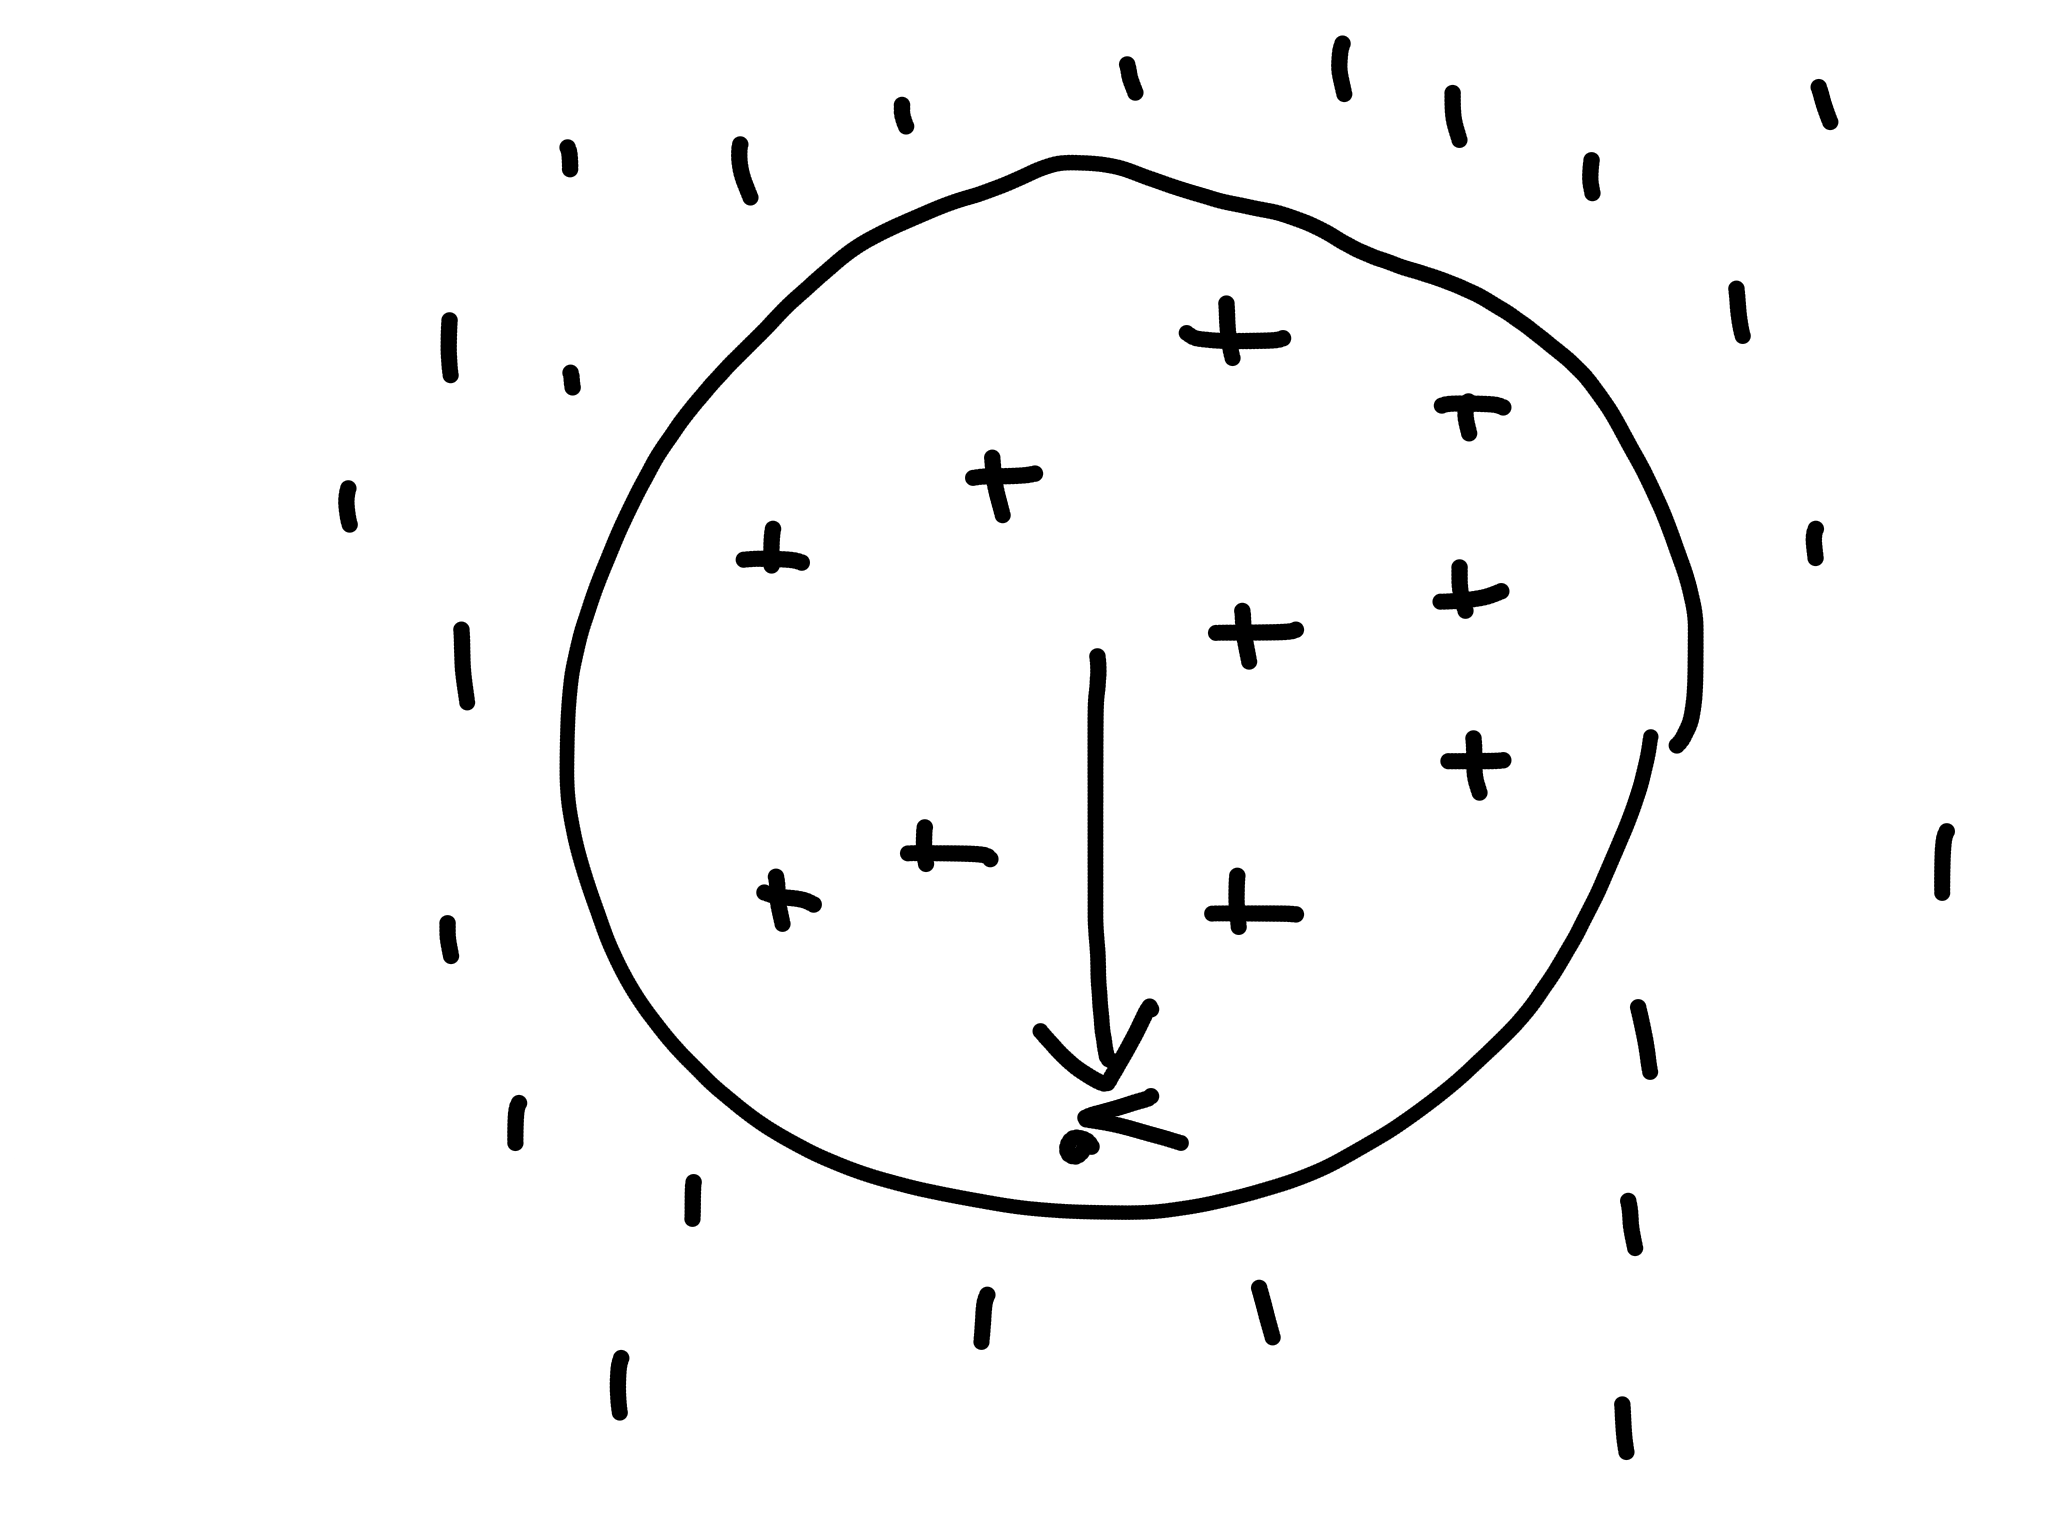
\includegraphics[angle=90,width=\linewidth]{../figures/ioncav.png}
\end{subfigure}

	\begin{subfigure}[b]{.4\marginparwidth}
	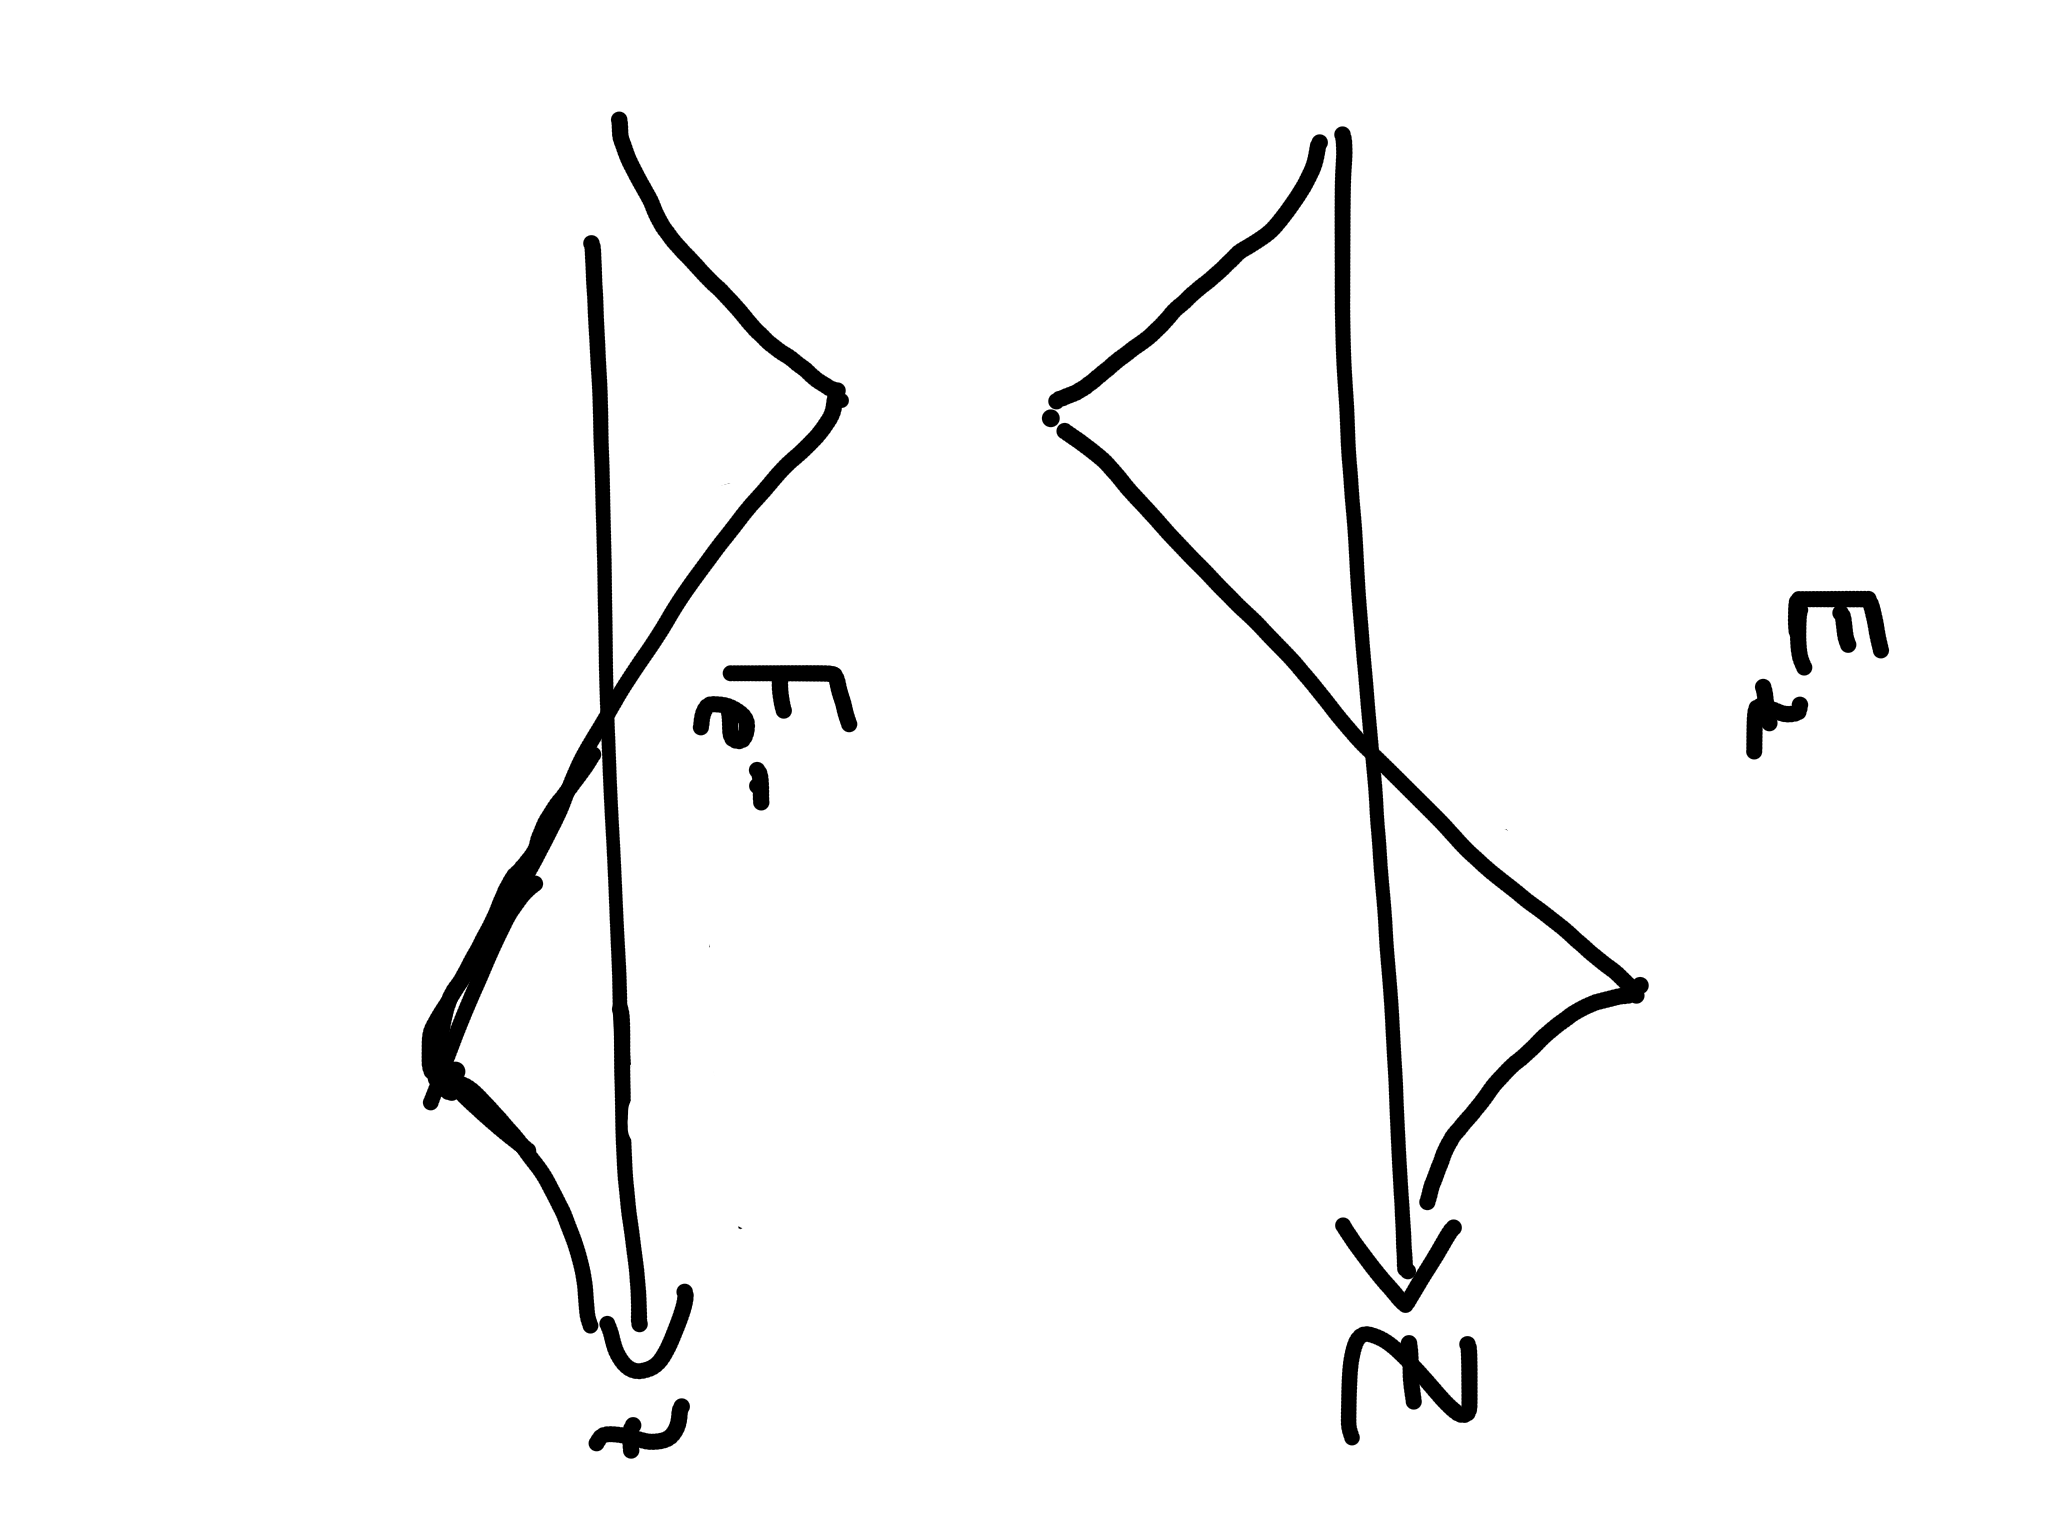
\includegraphics[angle=90,width=\linewidth]{../figures/ioncav2.png}
	\end{subfigure}
    \caption{The plasmon is what will accelerate the electrons. In the bubble
        regime it 
    can be modeled as an ion-sphere that moves through the background. It will
    create an electric field on the propogating axis that can accelerate
electrons}

\marginskip{90pt}
	\end{marginfigure}
    \subsection{1D Non-Relativistic (Cold Fluid)}
    In order to gain an intuition for the more complicated dynamics presented
    later, we will first consider the simplest situation: the interaction of
    light and plasma in a linear\sidenote{The linear refers to the fact that
        the intensity of light is small enough that the interaction can be
    treated perturbatively} regime. From radiowaves bouncing off of the
    ionosphere, to light reflecting off of a metal, light-plasma interactions
    are a common and well-studied phenomena. In constast to the phenomena of
    plasma reflection mentioned above, we will be dealing with a situation 
    where the EM wave propogates through the plasma.
    An important characteristic of the plasma that seperates the reflection
    from propogation case is the plasma frequency. If we look at the plasma
    dispersion relation in Figure \ref{fig:dispersion}, we can see that the
    plamsa simply won't support propogating waves that have a frequency less
    that it's natural frequency $\omega_p$. 


\begin{marginfigure}
    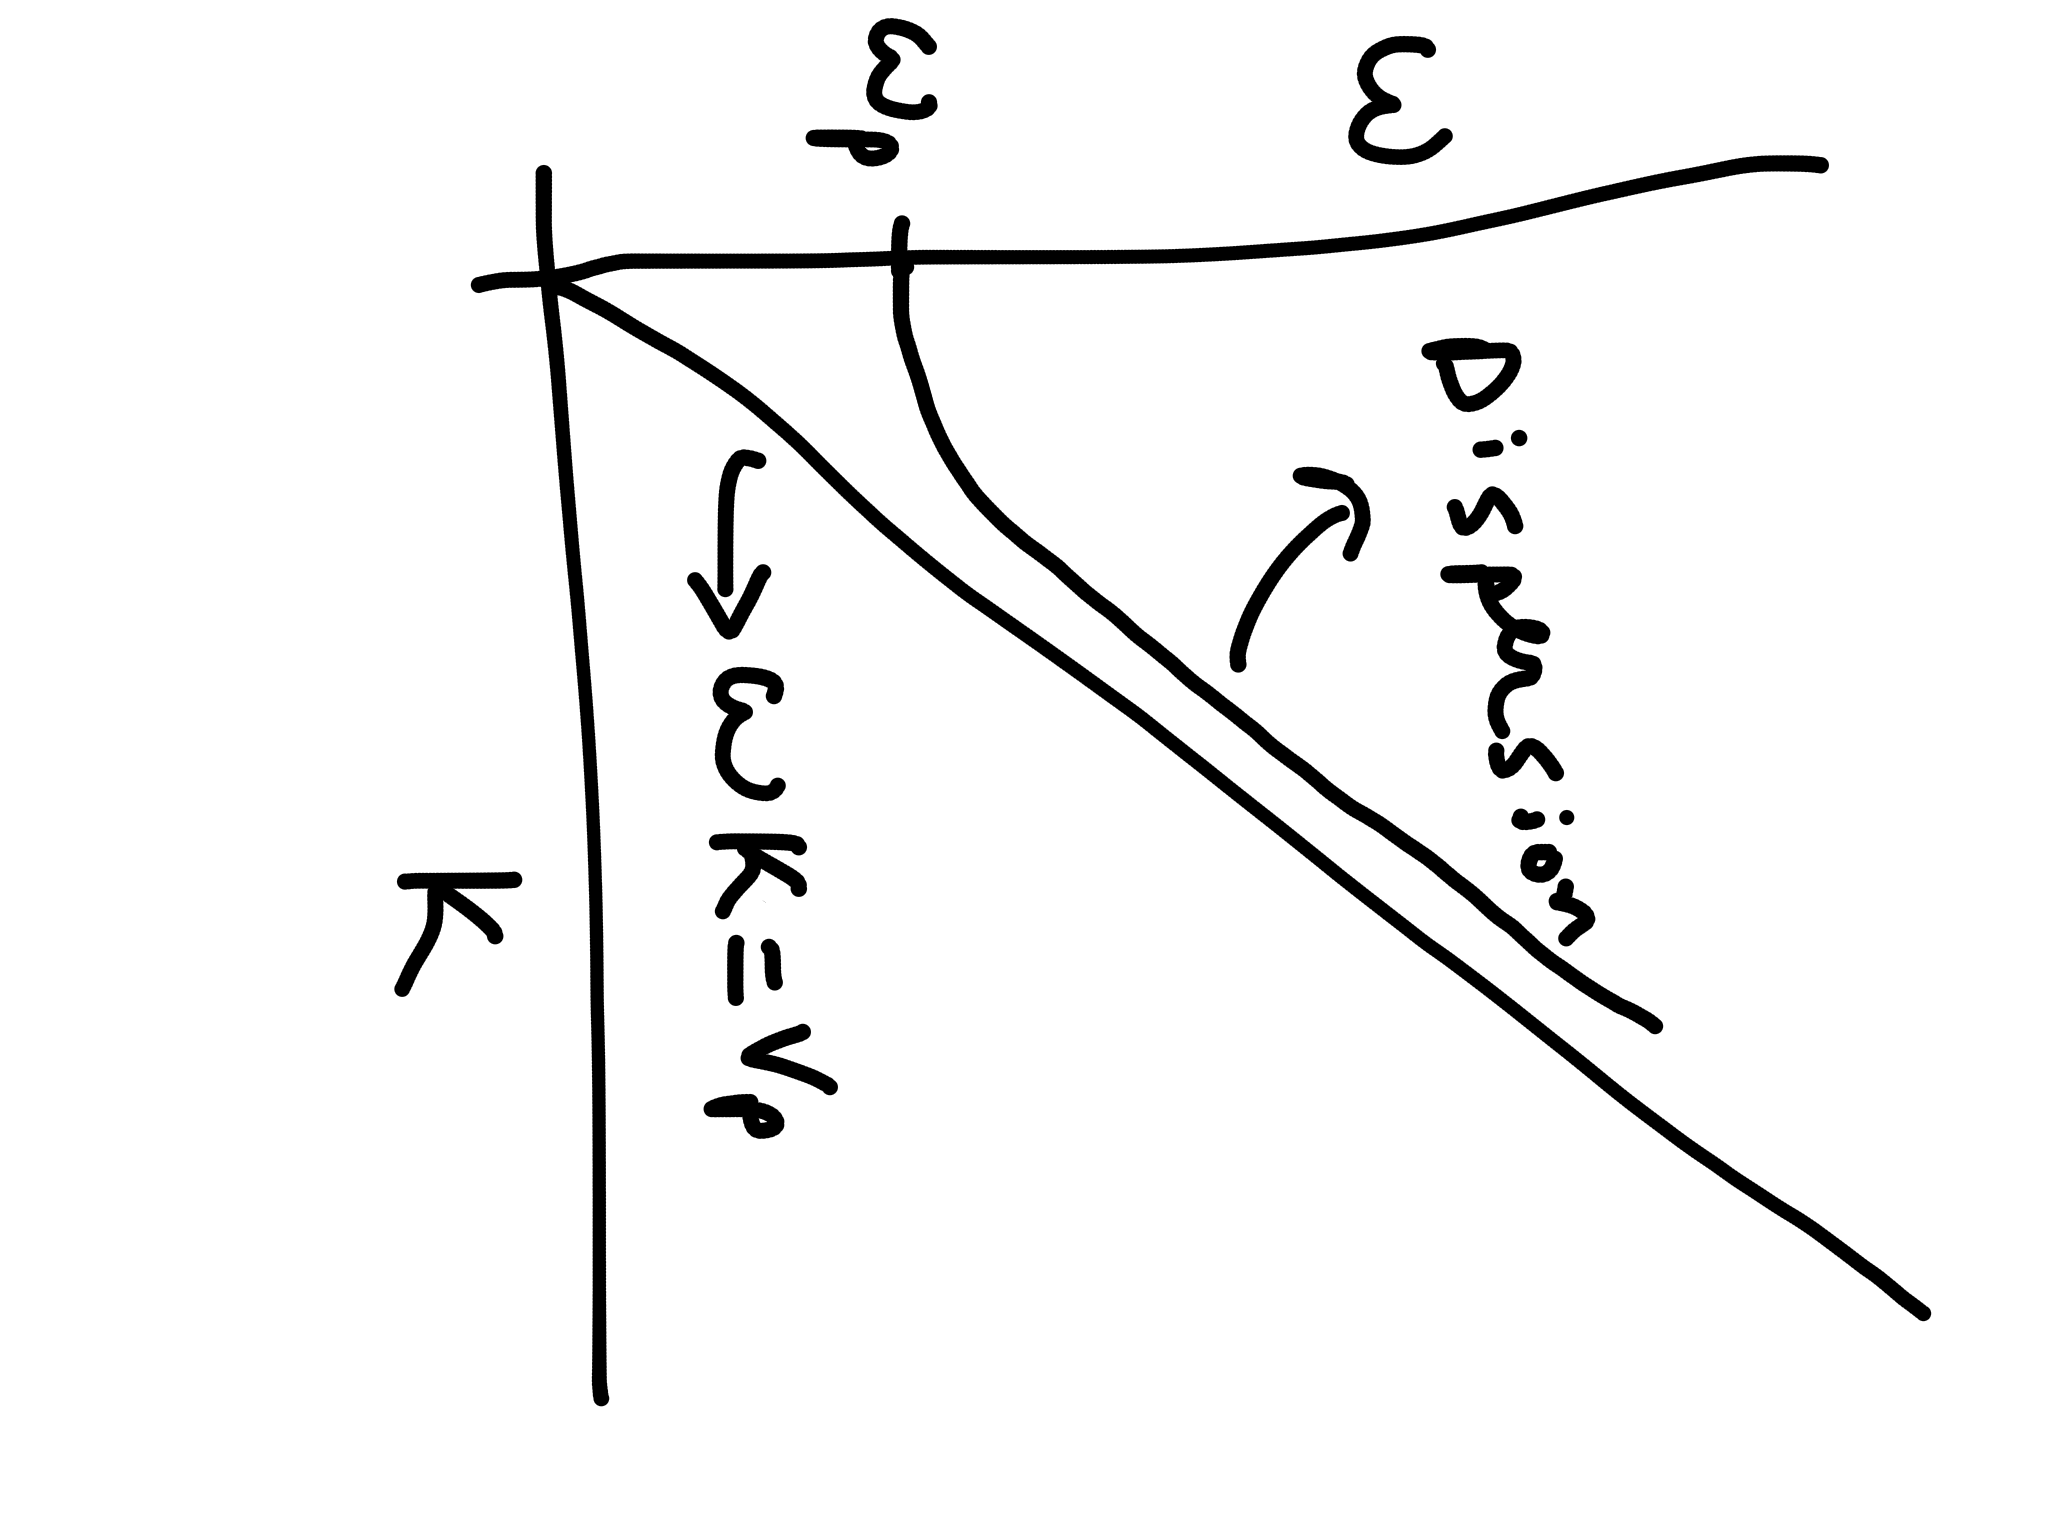
\includegraphics[angle=90, width =.6\marginparwidth]{../figures/disp.png}
    \caption{\label{fig:dispersion}The plasma disperion relation. Any EM waves that are propogating
        below the plasma frequency will be reflected (light reflecting from
        metal), if the EM wave is higher frequency, it can propogate through.}
    \end{marginfigure}

    The plasmas we are considering can be thought of as a fluid of electrons,
    mixed with a fluid of heavier ions. The difference in mass is important, as
    it means that we can essentialy negelect the ion motion. The electron fluid
    then will osscillate with it's natural frequency (it bears emphasizing that
    this will be a longitidinal density wave, called a plasmon). 

    When the high-intensity pulsed laser is incident on the plasma it will have
    two main effects: the first is to impart an acceleration perpendicular to
    the propogating axis\sidenote{This is due to the carrier accelerating the
        electrons. In the literature, this is refered to as the `quiver'
        momentum as it's net act is time-averaged to zero. It cannot be used to 
    excite a plasmon}; the second is to accelerate the electrons along the
    propogating axis. This second acceleration is due to the ponderomotive
    force, which is a second order effect that can be thought of as a force
 \begin{marginfigure}
    \centering
    \begin{subfigure}[b]{.75\marginparwidth}
    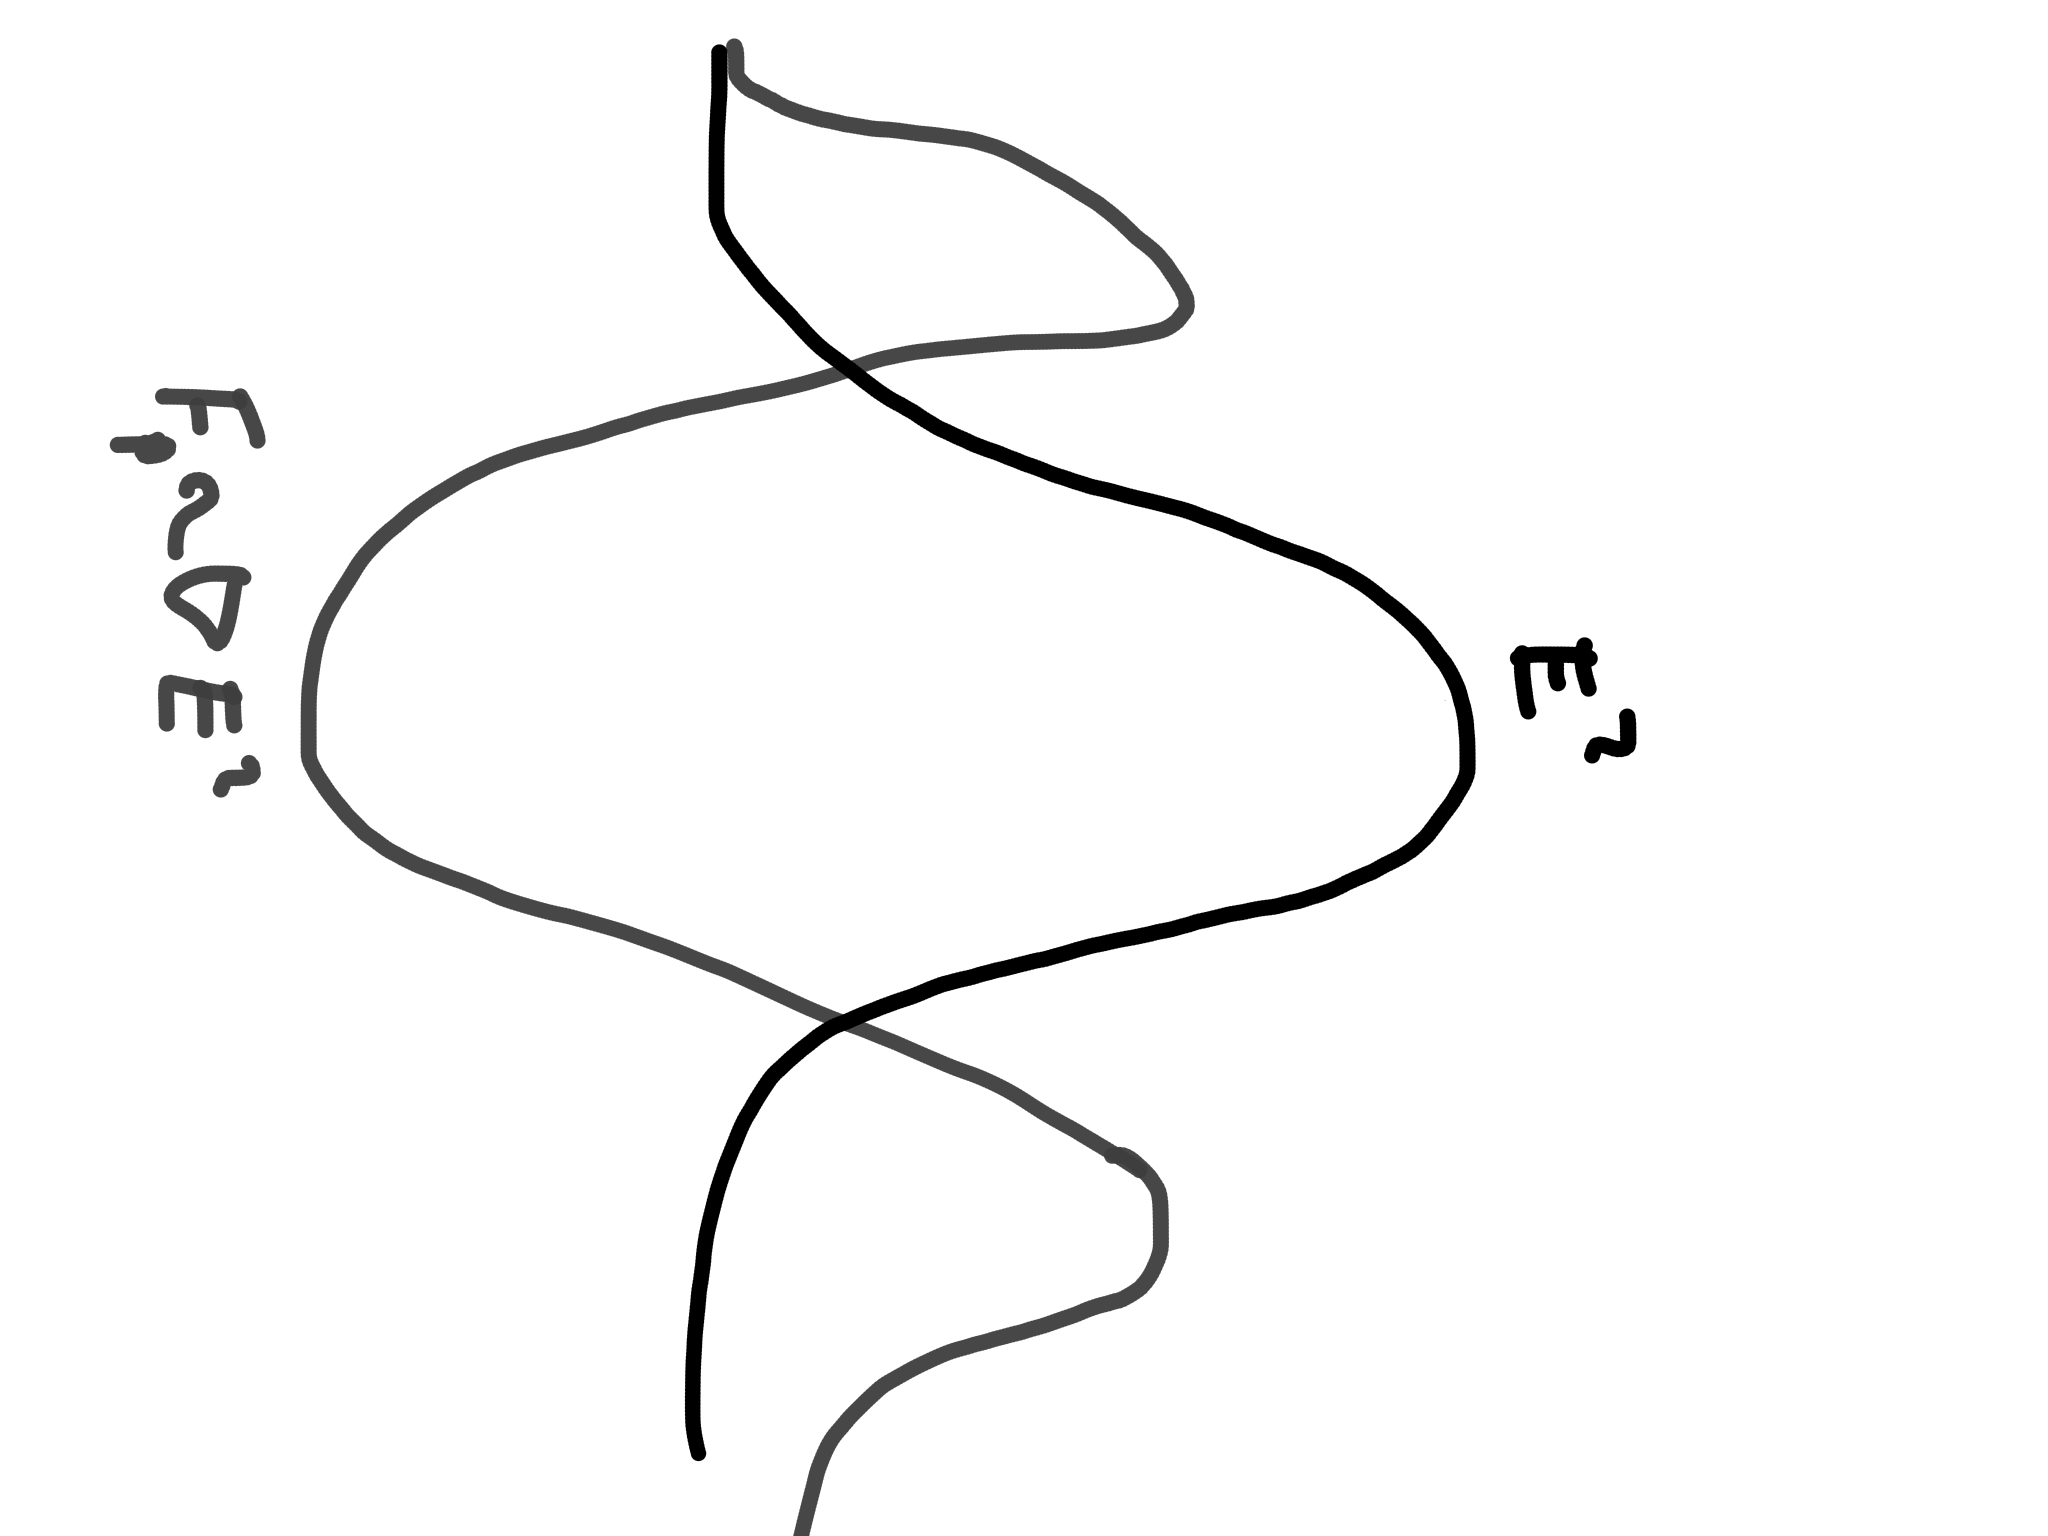
\includegraphics[angle=90,width=\linewidth]{../figures/pondforce.png}
\end{subfigure}

\begin{subfigure}[b]{.75\marginparwidth}
    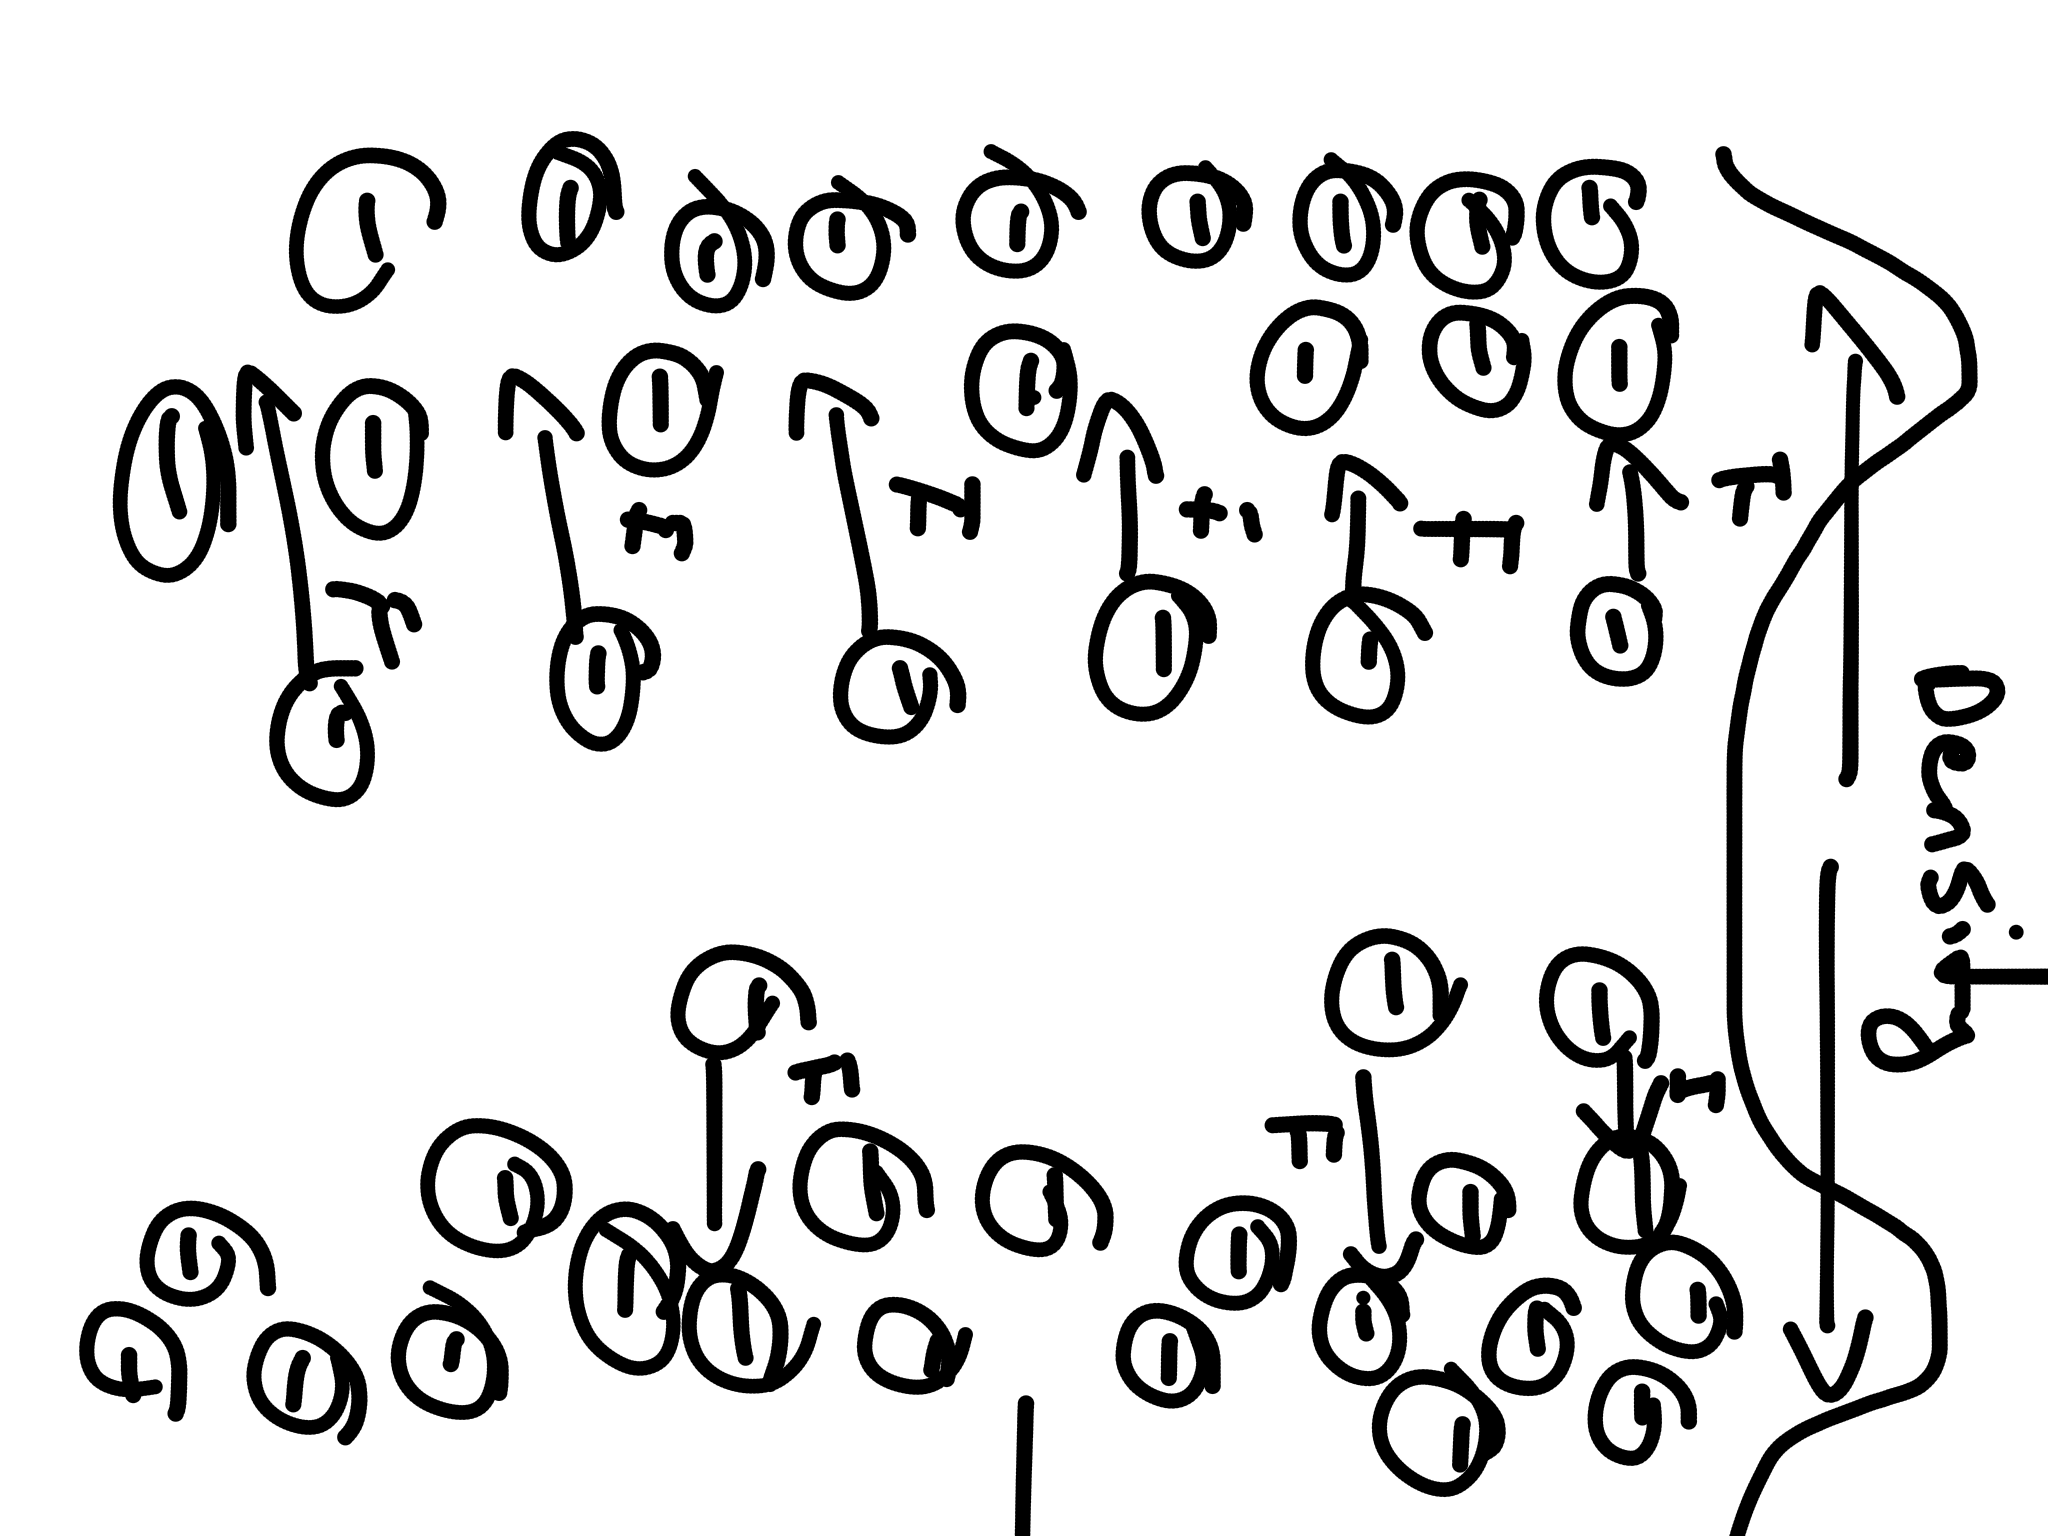
\includegraphics[width=\linewidth, angle=90]{../figures/ionback.png}
\end{subfigure}
\caption{The ponderomotive force can be thought of as the gradient of EM energy.
It will act to move electrons out of the central region of the laser pulse.}
\end{marginfigure}
   resulting from the gradient of electromagnetic energy in the laser pulse.


   The ponderomotive force will excite the co-propogating plasmon. 
   \begin{figure}[h!]
       \centering
       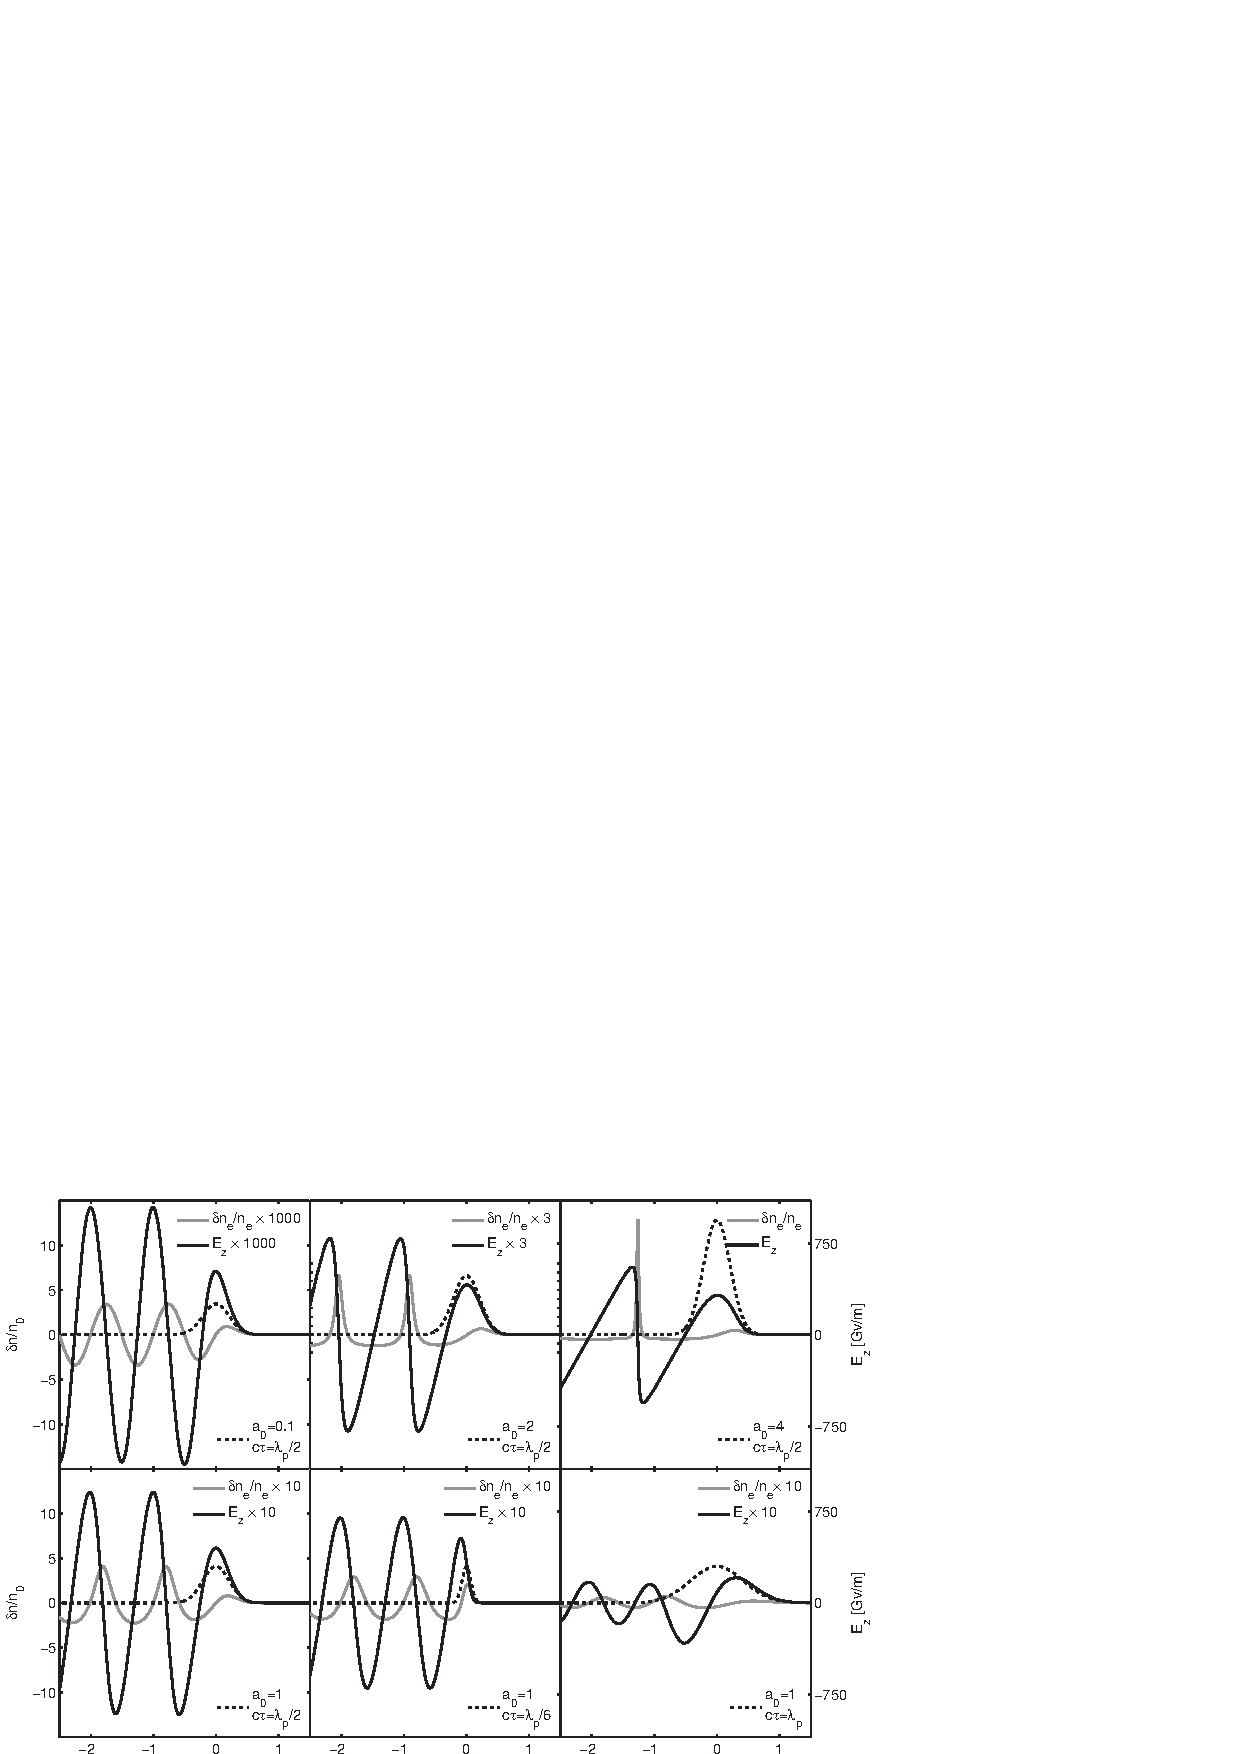
\includegraphics[width = .8\linewidth]{../figures/densityandewave.pdf}
       \caption{Showing plasmons generated with varying strengths of the peak
       amplitude of the laser pulse.\cite{genothesis}}
   \end{figure}
   In summary, we have discussed the mechanism of acceleration (longitudinal
   electric field produced by the density wave), and we have discussed how we
   create this mechanism within the plasma (high-intensity laser pushes
   electrons with the ponderomotive force.) Now, we have to discuss how the
   electrons are actually accelerated. Much like water waves, plasmons cannot
   accelerate objects unless two conditions are met\cite{PhysRevLett.113.085001}: the object needs to meet
   some phase-matching requirements, and the plasmon needs to be non-linear. 


   \subsection{Electron Trapping, Injection, and Acceleration}

    In order to be accelerated by the co-propogating electric field created by the
    plasmon, the electrons need to be travelling at some minimum speed. In the
    plasmon frame of reference, what an electron will see is, roughly, an
    ion-sphere. If we confine the electrons motion to 1D, then it can exhibit
    periodic motion about the centre of this sphere. 

    However, for this to work, the electron needs to have some minimum energy.
    Imagining a simple harmonic potential that is moving at some brisk speed $v_b >
    \sqrt{2 V_\mathrm{height of well}/m} $, we can see that an electron at rest will
    not be trapped: transforming to the potentials frame of reference, the electron
    will have too much energy to be trapped.
    This is quite similar to the case we are describing: however, we now have to
    consider that the electron's motion is going to be relativistic. In this case,
    the minimum energy an electron needs is given by \todo[inline]{need to add citation}:
    \begin{equation}
        \gamma_\mathrm{min} = \Delta \phi / (1+\beta_p) + \beta_p/(2 \Delta \phi)
    \end{equation}

    \todo[inline]{I'm not sure about adding this equation in. Probably take it out-- leave
        it at a general discussion and maybe show a plot of what a test electron's
    trajectory would look like.}

    For a very specific value of the accelerating electric field the background
    electrons that make up the density flucuations will actually meet the
    requirements to be trapped in this way. This gives rise to the phenomena of
    wavebreaking. In contrast to the perhaps more familiar example of water-wave's
    breaking, plasma wavebreaking is not a dispersion related phenomena. It is a
    non-linear effect, where the accelerating field created by the density
    flucuations of electrons in the plasma is strong enough to directly effect the
    density flucuations themselves.

    Wavebreaking is a useful phenomena for LWFA as it creates a larger field that
    can give more energy to the electrons. The phenomelogical differences between a
    linear plasmon and a wavebroken plasmon are show in Figure \todo[inline]{add figure}.

    {\em Trapping and accleration in nonlinear plasma waves was very useful-- a
        little terse. Mainly, they just guessed the hamiltonian for the system,
        plotted traj. around the fixed points and then said that the largest energy
        gain is by largest traj in phase space. (makes sense). Then they solve for
        the minimun kinetic energy a test electron would have on the largest traj.
        This then is the minimum energy required for an electron to be caught. I'm
        still not quite sure about some of the sublties about the phase (position)
    relationship to the energy.}
    \subsection{Electron Acceleration}
    The plasma bubble will set up a very high \si{\giga \electronvolt \per
    \centi \meter} acceleration field, however what will limit the total energy
    gain is how far the electron can be accelerated for. 
    There are three main lengths involved with accelerating the
    electrons.
    
    The first, $L_\mathrm{Dephasing}$ is analogous to what happens
    when a surfer outruns the wave they are on; no longer being accelerated,
    they slow down as their energy is dissapated to the waves. Similarly, electrons
    can outrun the plasma bubble. 

    The second, $L_\mathrm{Pulse Depletion}$, occurs because the interaction
    with of the laser-plasma will dissipate the energy of the initial laser
    pulse. The energy in the initial laser will be transfered to the plasma
    wake, where it will ultimately be disappaited as heat. 

    The third length, $L_\mathrm{Diffraction}$ is the most important, as it is
    the limiting length scale. This length scale is due to the inherent
    diffraction of lasers. In order to achieve the intense energies neccesary
    for the bubble regime, the lasers need to be focused down to a specific spot
    size. As soon as the minimum spot size is reached, the laser will begin to
    diffract, the length scale where the laser is approximately the spot size is
    the Rayleigh length. In a plasma this becomes more complicated, as the
    plasma can and will act like a lens. This leads to a feedback effect, where
    the intense laser pulse will change the plasma density, which in turn
    changes the intense laser pulse, and so on. The majority of effort in current wakefield accelerator  programs is to overcome this issue.

    In Figure \ref{fig:energy}, we can see the length scales multiplied by the
    accelerating electric field-- giving the total energy possible if an
    electron was accelerated over that distance. Clearly, the limiting length
    scale is diffraction.
    \begin{marginfigure}
        \begin{subfigure}[t]{\marginparwidth}
            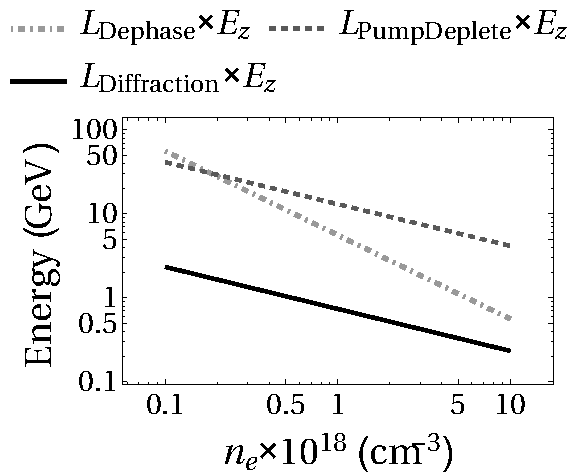
\includegraphics[width=\linewidth]{../figures/energy.pdf}
        \end{subfigure}
        \caption{The three length scales involved with accelerating electrons:
        $L_\mathrm{Dephase}$ where the electron outruns the wave, self-limiting
    the total energy gained; $L_\mathrm{Pump Depletion}$ where the incident
energy in the laser pulse is completely transfered to the wakefield, and the
laser can no longer sustain the bubble regime; and $L_\mathrm{Diffraction}$ the
inherent diffraction of the laser pulse. All lengths are scaled by an
accelerating field using parameters from the Texas
experiment\cite{Wang2013}, to show the total possible energy an electron
could gain.\label{fig:energy}}
    \end{marginfigure}


\section{Experimental Set-Up and State-of-the-Art}
In this review, we will focus on the experimental efforts of two groups, UT
Austin Texas, and University of California Berkeley. Although there are many
more groups doing interesting work in the field of LWFA, these two groups are
the main ones actively pursuing the goal of high-energy electron
accleration.
\begin{marginfigure}
	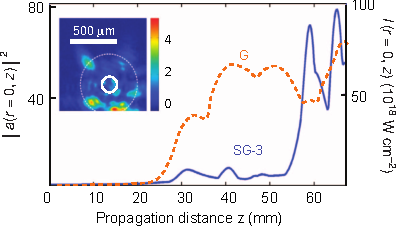
\includegraphics[width=\marginparwidth]{../figures/wakesimulation.pdf}
    \caption{Simulations done by the Texas group using the WAKE
        code showing clear features of self-focusing.\cite{Wang2013} As the
        normalized laser-intensity gets larger, the pulse is
        contracting--concentraing more of its energy over a smaller area.
        Interestingly, the self-focusing exhibits a periodic structure-- going
        through two cycles of diffraction-focusing for the super-gaussian
    pulse.\label{fig:propsim}}
\end{marginfigure}


\sidenote{Although, with the new high-energy laser laboratory
    system CILEX\cite{Cros20t427} soon coming online, it is probable that several European groups will be back in the race to high GeV electrons.}

The main limiting factor in laser-plasma-accleration is getting a larger
distance that the electrons can be accelerated by. Usually, the limiting factor
is the inherent diffraction of the laser pulse. Each of the two groups has a
unique strategy of overcoming this problem. 

The Texas group uses very high-intensity laser pulses and exploits the
phenomena of relativistic self-guiding to cancel out the inherent diffraction
of the laser. The Berkeley group uses low-intensity laser pulses and plasma waveguide channels to overcome the diffraction issue. A more in depth review of
each group is presented below.

\subsection{Texas: Or High-Intensity, Long Pulses with Relativistic Focussing}

In 2013, the Texas group reported a collumated beam of \SI{2}{\giga
\electronvolt}, which blew current records out of the
water\cite{Wang2013}.

Their approach used the new petawatt laser facility at UT Austin. The large
amplitudes that the laser was capable of generating placed them firmly in the
relativisitic self-guiding regime.
\begin{marginfigure}
	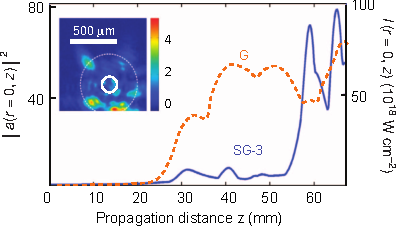
\includegraphics[width=\marginparwidth]{../figures/wakesimulation.pdf}
    \caption{Simulations done by the Texas group using the WAKE
        code showing clear features of self-focusing.\cite{Wang2013} As the
        normalized laser-intensity gets larger, the pulse is
        contracting--concentraing more of its energy over a smaller area.
        Interestingly, the self-focusing exhibits a periodic structure-- going
        through two cycles of diffraction-focusing for the super-gaussian
    pulse.\label{fig:propsim}}
\end{marginfigure}
Now, this is seperation text
\begin{figure*}[b!]
    \centering
	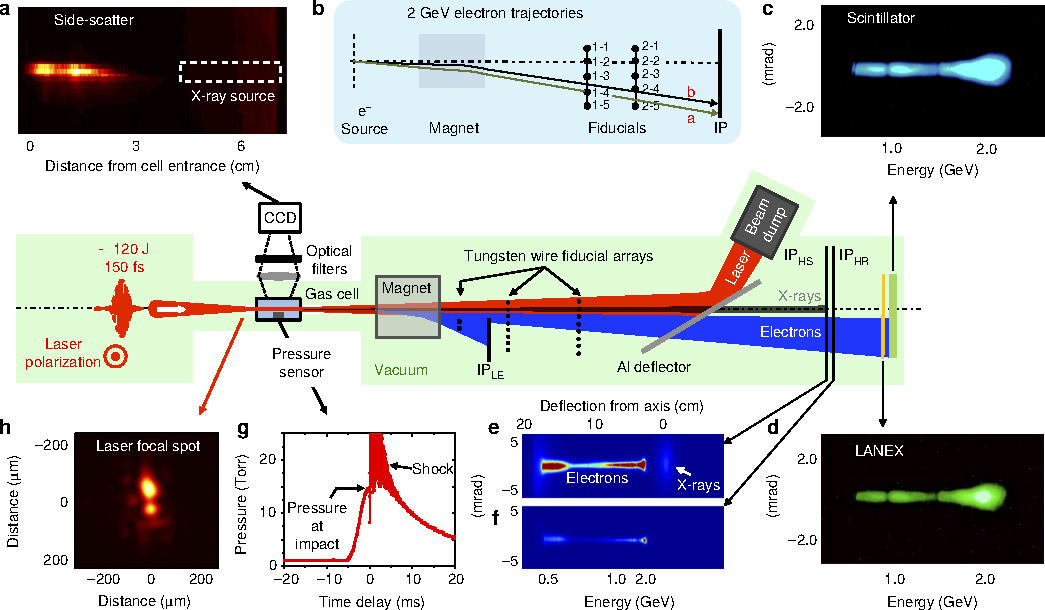
\includegraphics[width=500pt,height=250pt]{../figures/texasexplayout.pdf}
    \caption{The experimental setup of the Texas group.\cite{Wang2013} \em{This
    figure is reproduced from Nat. Commun. Vol. 4, 2013}}
\end{figure*}

The Texas group is now hard at work trying to find a strategy to increase the
energy of the electrons. Although their initial result is very promising, there
isn't a clear way forward. This is due to the very complicated dynamics of the
highly non-linear laser-plasma interaction that leads to self-focusing. As
shown in Figure \ref{fig:propsim}, the behaviour of the self-focusing is very
dependent on initial conditions (laser intensity, laser pulse shape, etc.). As
no analytic model can fully encompass its behaviour, numerical simulation is
required to understand the self-focusing behaviour required to produce
accleration lengths required for high energy electrons.

Their current work is focused on visualizing and understanding the propogation
of high-intensity laser light through their plasma, and they have developed
several novel techniques.

\todo[inline]{Expand on this-- quickly summarize the visualization thesis. Cite
a few of their more recent papers}

\subsection{Low-Intensity, Quasi-Linear Plasmas with Waveguides}
In 2014, the Berkeley group reported a collumated electron beam with peak
energy of \SI{4.2}{\giga \electronvolt}.

The Berkeley has, for a while now, pursued the strategy of low-intensity laser
pulses that are guided through channels. Their most current results use a
capillary discharge channel. 

The benefits over the Texas strategy is that they gain signifigantly on energy
conversion. Because they don't need to enter into the self-focusing regime,
they can use much less powerful lasers, and compensate by accelerating the
electrons over a larger distance. 
\section{Future Work and Outlook for the Field}
\section{Conclusion}
\begin{comment}
\subsection{The Need for Plasmas}
The reason that LPA has had such a resurgance is that it was only recently that 
laser technology was able to produce the electric field gradients neccesary. For 
instance, the laser used at UT-Austin in their LPA technology uses required a 
peak intensity of \SI{e18}{W.cm^{-2}} {\bf (not quite right, this is another 
group).}
It is tempting to ask why the plasma is needed at all when you have a laser 
capable of generating such high power-- why not just use the laser? In {\bf 
date} Woodward and Lauren proved that laser's cannot actually be used to 
accelerate particles, for much the same reason that boats only move up and down 
in linear ocean waves. {\bf maybe not the full story-- the ponderamotive force 
can't?}

The plasma acts as an intermediary, allowing the large electronic gradients 
present in a propogating high-intensity laser pulse to be transfered into a 
co-propogating longitudal wave. It is this longitudal wave that allows the 
electrons to be accelerated. In the section that follows, we will dicuss the 
physics behind this energy transfer in more depth.


\section{The Creation and Propogation of Plasmons and Bubbles}
The full theory required to describe the current state-of-the-art LPA technology 
is
too difficult to treat analytically, so the majority of theoretical research 
currently
being done in the field uses numerics. However, the basic physics involved with 
LPA technology
can be illustrated quite simply, which can be useful to build an intuition about 
the
processes that occur. In the following sections, we will review a basic physical 
model
of the laser plasma interaction.


\subsection{Linear Regime: Cold Fluid Equations}
To first order the plasma can be treated as a set of uncoupled harmonic 
oscillators. When the high-intensity, short-pulsed laser is incident, it will 
have two main actions: the first is to accelerate\footnote{The term used to 
describe this in plasma literature is `quiver', as the time-average motion 
amounts to zero because of the oscillitory nature of the radial electric 
field.l}
electrons along the radial electric field; the second is to accelerate electrons 
along the propogation direction due to the ponderomotive force. 

The ponderomotive force is due to the gradient in electromagnetic energy along a 
pulsed laser. {\bf show gaussian picture}. It will tend to create a `bubble', as 
it expels the lighter electrons from the laser pulse, leaving the heavier ions.

In our model, the ponderomotive force will act as a driving force on the plasma,
which has a natural oscillation rate $\omega_p$.  \begin{equation}
    \label{eq:linear density oscillation}
    \qty(\pdv[2]{}{t} +\omega_p^2) \frac{\delta n_e}{n_{e0}} = c^2 \laplacian{ 
    \frac{a^2}{2}}
\end{equation}

It is this density oscillation which creates an electric field through poisson's 
equation: $\vb{k}\dotproduct\vb{E} =\delta n_e/\epsilon$. It is this
longitudinally propogating electric field that will accelerate the electrons in 
the plasma.
 
{\it still need to mention resonance}

The propogating laser packet expels electrons from its local region, which acts
as a driving force to create a co-propogating density oscillation. This creates 
in effect a cavity of ions at moves at the phase velocity of the laser packet.  
This gives rise to an electric field gradient that will be able to accelerate 
electrons.
\section{Trapping Electrons}
In order to be accelerated by the co-propogating electric field created by the
plasmon, the electrons need to be travelling at some minimum speed. In the
plasmon frame of reference, what an electron will see is, roughly, an
ion-sphere. If we confine the electrons motion to 1D, then it can exhibit
periodic motion about the centre of this sphere. 

However, for this to work, the electron needs to have some minimum energy.
Imagining a simple harmonic potential that is moving at some brisk speed $v_b >
\sqrt{2 V_\mathrm{height of well}/m} $, we can see that an electron at rest will
not be trapped: transforming to the potentials frame of reference, the electron
will have too much energy to be trapped.
This is quite similar to the case we are describing: however, we now have to
consider that the electron's motion is going to be relativistic. In this case,
the minimum energy an electron needs is given by \todo[inline]{need to add citation}:
\begin{equation}
    \gamma_\mathrm{min} = \Delta \phi / (1+\beta_p) + \beta_p/(2 \Delta \phi)
\end{equation}

\todo[inline]{I'm not sure about adding this equation in. Probably take it out-- leave
    it at a general discussion and maybe show a plot of what a test electron's
trajectory would look like.}

For a very specific value of the accelerating electric field the background
electrons that make up the density flucuations will actually meet the
requirements to be trapped in this way. This gives rise to the phenomena of
wavebreaking. In contrast to the perhaps more familiar example of water-wave's
breaking, plasma wavebreaking is not a dispersion related phenomena. It is a
non-linear effect, where the accelerating field created by the density
flucuations of electrons in the plasma is strong enough to directly effect the
density flucuations themselves.

Wavebreaking is a useful phenomena for LWFA as it creates a larger field that
can give more energy to the electrons. The phenomelogical differences between a
linear plasmon and a wavebroken plasmon are show in Figure \todo[inline]{add figure}.

{\em Trapping and accleration in nonlinear plasma waves was very useful-- a
    little terse. Mainly, they just guessed the hamiltonian for the system,
    plotted traj. around the fixed points and then said that the largest energy
    gain is by largest traj in phase space. (makes sense). Then they solve for
    the minimun kinetic energy a test electron would have on the largest traj.
    This then is the minimum energy required for an electron to be caught. I'm
    still not quite sure about some of the sublties about the phase (position)
relationship to the energy.}
\end{comment}
\bibliography{../rep.bib}
\end{document}

